\documentclass[10pt]{article}
\usepackage[polish]{babel}
\usepackage[utf8]{inputenc}
\usepackage[T1]{fontenc}
\usepackage{graphicx}
\usepackage[export]{adjustbox}
\graphicspath{ {./images/} }
\usepackage{amsmath}
\usepackage{amsfonts}
\usepackage{amssymb}
\usepackage[version=4]{mhchem}
\usepackage{stmaryrd}
\usepackage{multirow}

\begin{document}
PLACÓWKA AKREDYTOWANA

\section*{KOD}
\begin{center}

\includegraphics[max width=\textwidth]{2024_11_21_8e981e1ab2c7e641f462g-01}
\end{center}

\section*{PESEL}
\begin{center}

\includegraphics[max width=\textwidth]{2024_11_21_8e981e1ab2c7e641f462g-01(1)}
\end{center}

PRÓBNY EGZAMIN MATURALNY

\section*{Z MATEMATYKI}
\section*{POZIOM PODSTAWOWY}
\begin{enumerate}
  \item Sprawdź, czy arkusz egzaminacyjny zawiera 16 stron (zadania 1-34). Ewentualny brak zgłoś przewodniczącemu zespołu nadzorującego próbny egzamin.
  \item Rozwiązania zadań i odpowiedzi wpisuj w miejscu na to przeznaczonym.
  \item Odpowiedzi do zadań zamkniętych (1-25) przenieś na kartę odpowiedzi, zaznaczając je w części karty przeznaczonej dla zdającego. Zamaluj - pola do tego przeznaczone. Błędne zaznaczenie otocz kółkiem i zaznacz właściwe.
  \item Pamiętaj, że pominięcie argumentacji lub istotnych obliczeń w rozwiązaniu zadania otwartego (26-34) może spowodować, że za to rozwiązanie nie będziesz mógł dostać pełnej liczby punktów.
  \item Pisz czytelnie i używaj tylko długopisu lub pióra z czarnym tuszem lub atramentem.
  \item Nie używaj korektora, a błędne zapisy wyraźnie przekreśl.
  \item Pamiętaj, że zapisy w brudnopisie nie będą oceniane.
  \item Możesz korzystać z zestawu wzorów matematycznych, cyrkla i linijki oraz kalkulatora.
  \item Na karcie odpowiedzi wpisz swój numer PESEL.
  \item Nie wpisuj żadnych znaków w części przeznaczonej dla egzaminatora.
\end{enumerate}

Marzec 2016

Czas pracy:\\
170 minut

\section*{Liczba punktów}
do uzyskania: 50

\section*{ZADANIA ZAMKNIETE}
W zadaniach od 1. do 25. wybierz i zaznacz na karcie odpowiedzi poprawna odpowiedź. Zadanie 1. (1 pkt)\\
Liczba \(\frac{\left(9 \cdot 5^{16}-5^{15}\right) \cdot 16^{3}}{4^{7} \cdot 625^{4}}\) równa jest\\
A. \(\frac{9}{4}\)\\
B. \(\frac{11}{5}\)\\
C. \(\frac{9}{2^{2} \cdot 5^{15}}\)\\
D. \(\frac{1}{2 \cdot 5^{12}}\)

Zadanie 2. (1 pkt)\\
Wyrażenie \((\mathrm{x}+4)(4-\mathrm{x})-(1-\mathrm{x})^{2}\) zapisać można w postaci\\
A. \(15+2 \mathrm{x}-2 \mathrm{x}^{2}\)\\
B. \(15-2 x\)\\
C. \(2 x-17\)\\
D. \(2 x^{2}-2 x-17\)

Zadanie 3. (1 pkt)\\
Poniżej przedstawiony jest wykres funkcji \(y=f(x)\).\\
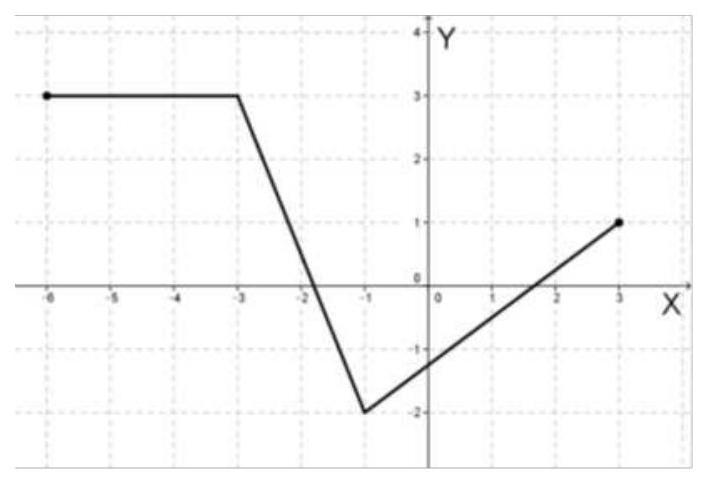
\includegraphics[max width=\textwidth, center]{2024_11_21_8e981e1ab2c7e641f462g-02(3)}

Wskaż wykres funkcji \(y=f(-x)\).\\
A.\\
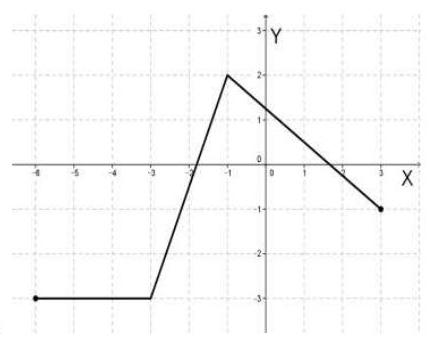
\includegraphics[max width=\textwidth, center]{2024_11_21_8e981e1ab2c7e641f462g-02(4)}\\
C.\\
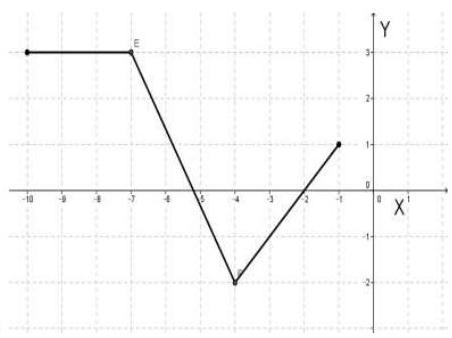
\includegraphics[max width=\textwidth, center]{2024_11_21_8e981e1ab2c7e641f462g-02(2)}\\
B.\\
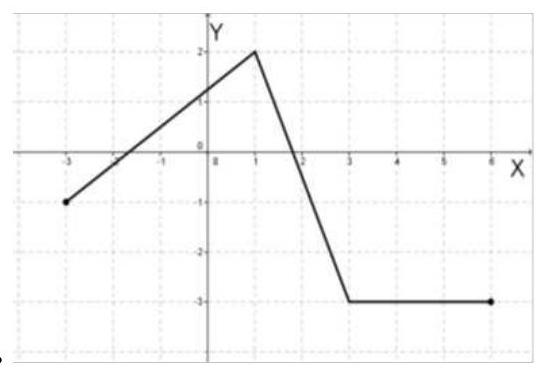
\includegraphics[max width=\textwidth, center]{2024_11_21_8e981e1ab2c7e641f462g-02(1)}\\
D.\\
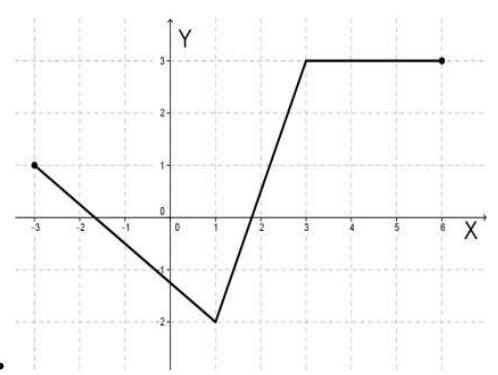
\includegraphics[max width=\textwidth, center]{2024_11_21_8e981e1ab2c7e641f462g-02}

\section*{Zadanie 4. (1 pkt)}
Ciąg 3, \(x^{2}, 27\) jest ciągiem geometrycznym, gdy\\
A. tylko \(x=-3\)\\
B. tylko \(x=3\)\\
C. \(x=-3 \operatorname{lub} x=3\)\\
D. \(x=-9 l u b x=9\)

\section*{BRUDNOPIS}
\begin{center}
\begin{tabular}{|c|c|c|c|c|c|c|c|c|c|c|c|c|c|c|c|c|c|c|c|c|c|c|c|}
\hline
 &  &  &  &  &  &  &  &  &  &  &  &  &  &  &  &  &  &  &  &  &  &  &  \\
\hline
 &  &  &  &  &  &  &  &  &  &  &  &  &  &  &  &  &  &  &  &  &  &  &  \\
\hline
 &  &  &  &  &  &  &  &  &  &  &  &  &  &  &  &  &  &  &  &  &  &  &  \\
\hline
 &  &  &  &  &  &  &  &  &  &  &  &  &  &  &  &  &  &  &  &  &  &  &  \\
\hline
 &  &  &  &  &  &  &  &  &  &  &  &  &  &  &  &  &  &  &  &  &  &  &  \\
\hline
 &  &  &  &  &  &  &  &  &  &  &  &  &  &  &  &  &  &  &  &  &  &  &  \\
\hline
 &  &  &  &  &  &  &  &  &  &  &  &  &  &  &  &  &  &  &  &  &  &  &  \\
\hline
 &  &  &  &  &  &  &  &  &  &  &  &  &  &  &  &  &  &  &  &  &  &  &  \\
\hline
 &  &  &  &  &  &  &  &  &  &  &  &  &  &  &  &  &  &  &  &  &  &  &  \\
\hline
 &  &  &  &  &  &  &  &  &  &  &  &  &  &  &  &  &  &  &  &  &  &  &  \\
\hline
 &  &  &  &  &  &  &  &  &  &  &  &  &  &  &  &  &  &  &  &  &  &  &  \\
\hline
 &  &  &  &  &  &  &  &  &  &  &  &  &  &  &  &  &  &  &  &  &  &  &  \\
\hline
 &  &  &  &  &  &  &  &  &  &  &  &  &  &  &  &  &  &  &  &  &  &  &  \\
\hline
 &  &  &  &  &  &  &  &  &  &  &  &  &  &  &  &  &  &  &  &  &  &  &  \\
\hline
 &  &  &  &  &  &  &  &  &  &  &  &  &  &  &  &  &  &  &  &  &  &  &  \\
\hline
 &  &  &  &  &  &  &  &  &  &  &  &  &  &  &  &  &  &  &  &  &  &  &  \\
\hline
 &  &  &  &  &  &  &  &  &  &  &  &  &  &  &  &  &  &  &  &  &  &  &  \\
\hline
 &  &  &  &  &  &  &  &  &  &  &  &  &  &  &  &  &  &  &  &  &  &  &  \\
\hline
 &  &  &  &  &  &  &  &  &  &  &  &  &  &  &  &  &  &  &  &  &  &  &  \\
\hline
 &  &  &  &  &  &  &  &  &  &  &  &  &  &  &  &  &  &  &  &  &  &  &  \\
\hline
 &  &  &  &  &  &  &  &  &  &  &  &  &  &  &  &  &  &  &  &  &  &  &  \\
\hline
 &  &  &  &  &  &  &  &  &  &  &  &  &  &  &  &  &  &  &  &  &  &  &  \\
\hline
 &  &  &  &  &  &  &  &  &  &  &  &  &  &  &  &  &  &  &  &  &  &  &  \\
\hline
 &  &  &  &  &  &  &  &  &  &  &  &  &  &  &  &  &  &  &  &  &  &  &  \\
\hline
 &  &  &  &  &  &  &  &  &  &  &  &  &  &  &  &  &  &  &  &  &  &  &  \\
\hline
 &  &  &  &  &  &  &  &  &  &  &  &  &  &  &  &  &  &  &  &  &  &  &  \\
\hline
 &  &  &  &  &  &  &  &  &  &  &  &  &  &  &  &  &  &  &  &  &  &  &  \\
\hline
 &  &  &  &  &  &  &  &  &  &  &  &  &  &  &  &  &  &  &  &  &  &  &  \\
\hline
 &  &  &  &  &  &  &  &  &  &  &  &  &  &  &  &  &  &  &  &  &  &  &  \\
\hline
 &  &  &  &  &  &  &  &  &  &  &  &  &  &  &  &  &  &  &  &  &  &  &  \\
\hline
 &  &  &  &  &  &  &  &  &  &  &  &  &  &  &  &  &  &  &  &  &  &  &  \\
\hline
 &  &  &  &  &  &  &  &  &  &  &  &  &  &  &  &  &  &  &  &  &  &  &  \\
\hline
 &  &  &  &  &  &  &  &  &  &  &  &  &  &  &  &  &  &  &  &  &  &  &  \\
\hline
 &  &  &  &  &  &  &  &  &  &  &  &  &  &  &  &  &  &  &  &  &  &  &  \\
\hline
 &  &  &  &  &  &  &  &  &  &  &  &  &  &  &  &  &  &  &  &  &  &  &  \\
\hline
 &  &  &  &  &  &  &  &  &  &  &  &  &  &  &  &  &  &  &  &  &  &  &  \\
\hline
 &  &  &  &  &  &  &  &  &  &  &  &  &  &  &  &  &  &  &  &  &  &  &  \\
\hline
 &  &  &  &  &  &  &  &  &  &  &  &  &  &  &  &  &  &  &  &  &  &  &  \\
\hline
 &  &  &  &  &  &  &  &  &  &  &  &  &  &  &  &  &  &  &  &  &  &  &  \\
\hline
 &  &  &  &  &  &  &  &  &  &  &  &  &  &  &  &  &  &  &  &  &  &  &  \\
\hline
 &  &  &  &  &  &  &  &  &  &  &  &  &  &  &  &  &  &  &  &  &  &  &  \\
\hline
 &  &  &  &  &  &  &  &  &  &  &  &  &  &  &  &  &  &  &  &  &  &  &  \\
\hline
 &  &  &  &  &  &  &  &  &  &  &  &  &  &  &  &  &  &  &  &  &  &  &  \\
\hline
\end{tabular}
\end{center}

\section*{Zadanie 5. (1 pkt)}
Kąt \(\alpha\) jest ostry i \(\cos \alpha=\frac{\sqrt{5}}{3}\). Wówczas\\
A. \(\operatorname{tg} \alpha=\frac{4 \sqrt{5}}{5}\)\\
B. \(\operatorname{tg} \alpha=\frac{\sqrt{5}}{2}\)\\
C. \(\operatorname{tg} \alpha=\frac{2 \sqrt{5}}{5}\)\\
D. \(\operatorname{tg} \alpha=\frac{2}{3}\)

Zadanie 6. (1 pkt)\\
Obwód kwadratu, którego przeciwległe wierzchołki mają współrzędne \(A=(-3,5)\) i \(C=(5,1)\) jest równy\\
A. \(2 \sqrt{10}\)\\
B. \(4 \sqrt{5}\)\\
C. \(8 \sqrt{10}\)\\
D. \(16 \sqrt{5}\)

Zadanie 7. (1 pkt)\\
Dane są dwa okręgi styczne wewnętrznie o promieniach \(r_{1}=10 \mathrm{cmi} r_{2}=4 \mathrm{~cm}\). Zatem odległość między ich środkami jest równa\\
A. 2 cm\\
B. 6 cm\\
C. 8 cm\\
D. 14 cm

Zadanie 8. (1 pkt)\\
Rozwiązaniem równania \(\frac{(x-2)(x+3)}{x^{2}-2 x}=0\) jest\\
A. \(x=2 i x=-3\)\\
B. tylko \(x=2\)\\
C. tylko \(x=-3\)\\
D. \(x=0 i x=2\)

\section*{Zadanie 9. (1 pkt)}
Długość tworzącej stożka jest równa 6, a obwód jego podstawy wynosi \(6 \sqrt{3}\). Kąt rozwarcia tego stożka ma miarę\\
A. \(30^{\circ}\)\\
B. \(60^{\circ}\)\\
C. \(90^{\circ}\)\\
D. \(120^{\circ}\)

Zadanie 10. (1 pkt)\\
Średnia arytmetyczna zestawu danych \(11,1,5,9, x, 3,7,12\) o medianie 7,5 jest równa\\
A. 8\\
B. 7,5\\
C. 7\\
D. 6,75

Zadanie 11. (1 pkt)\\
Suma wyrazów ciągu wyraża się wzorem \(S_{n}=2 n^{2}-4 n\), zatem\\
A. \(a_{2}=-2\)\\
B. \(a_{2}=-1\)\\
C. \(a_{2}=0\)\\
D. \(a_{2}=2\)

Zadanie 12. (1 pkt)\\
Na rysunku przedstawiono wykres funkcji liniowej \(f(x)=a x+b\). Zatem:\\
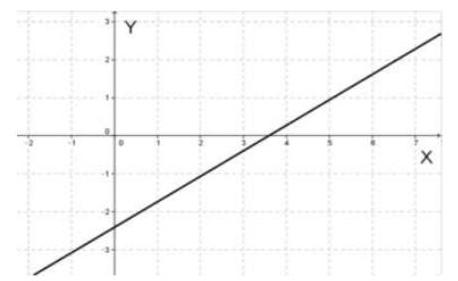
\includegraphics[max width=\textwidth, center]{2024_11_21_8e981e1ab2c7e641f462g-04}\\
A. \(a>0 i b>0\)\\
B. \(a<0 i b<0\)\\
C. \(a>0 i b<0\)\\
D. \(a<0 i b>0\)

\section*{BRUDNOPIS}
\begin{center}
\begin{tabular}{|c|c|c|c|c|c|c|c|c|c|c|c|c|c|c|c|c|c|c|c|c|c|c|c|}
\hline
 &  &  &  &  &  &  &  &  &  &  &  &  &  &  &  &  &  &  &  &  &  &  &  \\
\hline
 &  &  &  &  &  &  &  &  &  &  &  &  &  &  &  &  &  &  &  &  &  &  &  \\
\hline
 &  &  &  &  &  &  &  &  &  &  &  &  &  &  &  &  &  &  &  &  &  &  &  \\
\hline
 &  &  &  &  &  &  &  &  &  &  &  &  &  &  &  &  &  &  &  &  &  &  &  \\
\hline
 &  &  &  &  &  &  &  &  &  &  &  &  &  &  &  &  &  &  &  &  &  &  &  \\
\hline
 &  &  &  &  &  &  &  &  &  &  &  &  &  &  &  &  &  &  &  &  &  &  &  \\
\hline
 &  &  &  &  &  &  &  &  &  &  &  &  &  &  &  &  &  &  &  &  &  &  &  \\
\hline
 &  &  &  &  &  &  &  &  &  &  &  &  &  &  &  &  &  &  &  &  &  &  &  \\
\hline
 &  &  &  &  &  &  &  &  &  &  &  &  &  &  &  &  &  &  &  &  &  &  &  \\
\hline
 &  &  &  &  &  &  &  &  &  &  &  &  &  &  &  &  &  &  &  &  &  &  &  \\
\hline
 &  &  &  &  &  &  &  &  &  &  &  &  &  &  &  &  &  &  &  &  &  &  &  \\
\hline
 &  &  &  &  &  &  &  &  &  &  &  &  &  &  &  &  &  &  &  &  &  &  &  \\
\hline
 &  &  &  &  &  &  &  &  &  &  &  &  &  &  &  &  &  &  &  &  &  &  &  \\
\hline
 &  &  &  &  &  &  &  &  &  &  &  &  &  &  &  &  &  &  &  &  &  &  &  \\
\hline
 &  &  &  &  &  &  &  &  &  &  &  &  &  &  &  &  &  &  &  &  &  &  &  \\
\hline
 &  &  &  &  &  &  &  &  &  &  &  &  &  &  &  &  &  &  &  &  &  &  &  \\
\hline
 &  &  &  &  &  &  &  &  &  &  &  &  &  &  &  &  &  &  &  &  &  &  &  \\
\hline
 &  &  &  &  &  &  &  &  &  &  &  &  &  &  &  &  &  &  &  &  &  &  &  \\
\hline
 &  &  &  &  &  &  &  &  &  &  &  &  &  &  &  &  &  &  &  &  &  &  &  \\
\hline
 &  &  &  &  &  &  &  &  &  &  &  &  &  &  &  &  &  &  &  &  &  &  &  \\
\hline
 &  &  &  &  &  &  &  &  &  &  &  &  &  &  &  &  &  &  &  &  &  &  &  \\
\hline
 &  &  &  &  &  &  &  &  &  &  &  &  &  &  &  &  &  &  &  &  &  &  &  \\
\hline
 &  &  &  &  &  &  &  &  &  &  &  &  &  &  &  &  &  &  &  &  &  &  &  \\
\hline
 &  &  &  &  &  &  &  &  &  &  &  &  &  &  &  &  &  &  &  &  &  &  &  \\
\hline
 &  &  &  &  &  &  &  &  &  &  &  &  &  &  &  &  &  &  &  &  &  &  &  \\
\hline
 &  &  &  &  &  &  &  &  &  &  &  &  &  &  &  &  &  &  &  &  &  &  &  \\
\hline
 &  &  &  &  &  &  &  &  &  &  &  &  &  &  &  &  &  &  &  &  &  &  &  \\
\hline
 &  &  &  &  &  &  &  &  &  &  &  &  &  &  &  &  &  &  &  &  &  &  &  \\
\hline
 &  &  &  &  &  &  &  &  &  &  &  &  &  &  &  &  &  &  &  &  &  &  &  \\
\hline
 &  &  &  &  &  &  &  &  &  &  &  &  &  &  &  &  &  &  &  &  &  &  &  \\
\hline
 &  &  &  &  &  &  &  &  &  &  &  &  &  &  &  &  &  &  &  &  &  &  &  \\
\hline
 &  &  &  &  &  &  &  &  &  &  &  &  &  &  &  &  &  &  &  &  &  &  &  \\
\hline
 &  &  &  &  &  &  &  &  &  &  &  &  &  &  &  &  &  &  &  &  &  &  &  \\
\hline
 &  &  &  &  &  &  &  &  &  &  &  &  &  &  &  &  &  &  &  &  &  &  &  \\
\hline
 &  &  &  &  &  &  &  &  &  &  &  &  &  &  &  &  &  &  &  &  &  &  &  \\
\hline
 &  &  &  &  &  &  &  &  &  &  &  &  &  &  &  &  &  &  &  &  &  &  &  \\
\hline
 &  &  &  &  &  &  &  &  &  &  &  &  &  &  &  &  &  &  &  &  &  &  &  \\
\hline
 &  &  &  &  &  &  &  &  &  &  &  &  &  &  &  &  &  &  &  &  &  &  &  \\
\hline
 &  &  &  &  &  &  &  &  &  &  &  &  &  &  &  &  &  &  &  &  &  &  &  \\
\hline
 &  &  &  &  &  &  &  &  &  &  &  &  &  &  &  &  &  &  &  &  &  &  &  \\
\hline
 &  &  &  &  &  &  &  &  &  &  &  &  &  &  &  &  &  &  &  &  &  &  &  \\
\hline
 &  &  &  &  &  &  &  &  &  &  &  &  &  &  &  &  &  &  &  &  &  &  &  \\
\hline
 &  &  &  &  &  &  &  &  &  &  &  &  &  &  &  &  &  &  &  &  &  &  &  \\
\hline
 &  &  &  &  &  &  &  &  &  &  &  &  &  &  &  &  &  &  &  &  &  &  &  \\
\hline
\end{tabular}
\end{center}

Zadanie 13. (1 pkt)\\
Punkt \(P=(-8,15)\) znajduje się na końcowym ramieniu kąta \(\alpha\). Wówczas\\
A. \(\cos \alpha=-\frac{8}{17}\)\\
B. \(\cos \alpha=-\frac{8}{15}\)\\
C. \(\cos \alpha=\frac{8}{17}\)\\
D. \(\cos \alpha=\frac{15}{17}\)

Zadanie 14. (1 pkt)\\
Punkt \(O\) jest środkiem okręgu. Kąt środkowy \(\alpha\) ma miarę\\
A. \(50^{\circ}\)\\
B. \(100^{\circ}\)\\
C. \(130^{\circ}\)\\
D. \(260^{\circ}\)

Zadanie 15. (1 pkt)\\
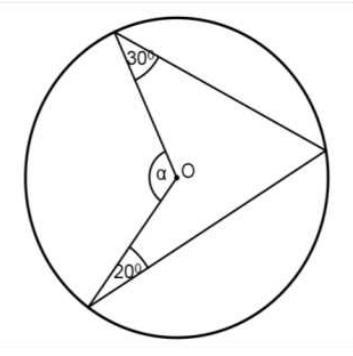
\includegraphics[max width=\textwidth, center]{2024_11_21_8e981e1ab2c7e641f462g-06}

Pole równoległoboku o bokach długości 6 cm i 10 cm i kącie rozwartym o mierze \(\alpha=120^{\circ}\) jest równe\\
A. \(30 \sqrt{3} \mathrm{~cm}^{2}\)\\
B. \(30 \mathrm{~cm}^{2}\)\\
C. \(15 \sqrt{3} \mathrm{~cm}^{2}\)\\
D. \(15 \mathrm{~cm}^{2}\)

Zadanie 16. (1pkt)\\
Równanie prostej prostopadłej do prostej \(2 x+y-3=0\) i przechodzącej przez punkt \(P=(4,-2)\) ma postać\\
A. \(y=\frac{1}{2} x+3\)\\
B. \(y=\frac{1}{2} x-4\)\\
C. \(y=-\frac{1}{2} x\)\\
D. \(y=2 x-10\)

Zadanie 17. (1 pkt)\\
Dany jest wykres funkcji \(y=f(x)\).\\
Dziedziną D i zbiorem wartości ZW tej funkcji jest\\
A. \(D=\langle-2,4), Z W=(-5,6\rangle\)\\
B. \(D=\langle-5,6\rangle, Z W=\langle-2,4\rangle\)\\
C. \(D=(-5,6\rangle, Z W=\langle-2,4)\)\\
D. \(D=\langle-2,4\rangle, Z W=\langle-5,6\rangle\)

Zadanie 18. (1 pkt)\\
Przekrojem prostopadłościanu zawierającym przekątną podstawy i przekątne sąsiednich ścian bocznych wychodzących z tego samego wierzchołka jest\\
A. kwadrat\\
B. prostokąt\\
C. trójkąt\\
D. trapez

Zadanie 19. (1 pkt)\\
Ania wyjeżdżając na wakacje zamknęła walizkę za pomocą kodu czterocyfrowego.\\
Pamiętała, że druga liczba jest liczbą pierwszą mniejszą od 7, trzecia jest liczbą nieparzystą, a czwarta to 5, ale zapomniała pierwszej liczby. Ile maksymalnie prób musi wykonać, aby otworzyć walizkę?\\
A. \(9 \cdot 4 \cdot 5 \cdot 5\)\\
B. \(10 \cdot 3 \cdot 5 \cdot 1\)\\
C. \(10 \cdot 4 \cdot 5 \cdot 1\)\\
D. \(9 \cdot 3 \cdot 5 \cdot 5\)

\section*{BRUDNOPIS}
\begin{center}

\includegraphics[max width=\textwidth]{2024_11_21_8e981e1ab2c7e641f462g-07}
\end{center}

Zadanie 20. (1 pkt)\\
Największa wartość funkcji kwadratowej \(f(x)=-x^{2}+6 x-5 \mathrm{w}\) przedziale \(\langle-2,4\rangle\) jest równa\\
A. 35\\
B. 22\\
C. 4\\
D. 3

Zadanie 21. (1 pkt)\\
Ilustracją graficzną zbioru rozwiązań nierówności \(\frac{x+2}{2}-\frac{x-1}{4}<\frac{3}{4} x \quad\) jest przedział\\
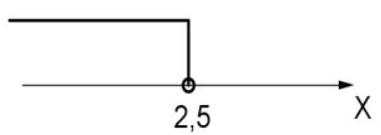
\includegraphics[max width=\textwidth, center]{2024_11_21_8e981e1ab2c7e641f462g-08}\\
A.\\
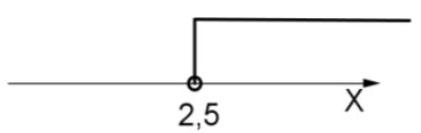
\includegraphics[max width=\textwidth, center]{2024_11_21_8e981e1ab2c7e641f462g-08(1)}\\
B.

Zadanie 22. (1 pkt)\\
Cena towaru z 22\% podatkiem VAT wynosi 183 zł. Cena tego towaru z 7\% podatkiem VAT jest równa\\
A. \(160,50 \mathrm{z}\)\\
B. \(195,81 \mathrm{zł}\)\\
C. 210,45 zł\\
D. \(223,26 \mathrm{zł}\)

Zadanie 23. (1 pkt)\\
Dany jest fragment wykresu pewnej funkcji kwadratowej \(y=f(x)\). Funkcja ta ma wzór\\
A. \(f(x)=-2 x^{2}+12 x-16\)\\
B. \(f(x)=2 x^{2}+12 x+16\)\\
C. \(f(x)=2 x^{2}-12 x-1\)\\
D. \(f(x)=-2 x^{2}-12 x-16\)

Zadanie 24. (1 pkt)\\
Liczba \(\log _{5} 8-3 \log _{5} 2\) jest równa\\
A. \(\log _{5} 56\)\\
B. \(\log _{5} \frac{16}{6}\)\\
C. \(\log _{5} 1\)\\
D. \(3 \log _{5} 2\)

Zadanie 25. (1 pkt)\\
Wzór ogólny ciągu arytmetycznego, w którym \(a_{3}=30 i a_{41}=524\), to\\
A. \(a_{n}=13 n-9\)\\
B. \(a_{n}=13 n+4\)\\
C. \(a_{n}=52 n-52\)\\
D. \(a_{n}=52 n\)

\section*{BRUDNOPIS}
\begin{center}
\begin{tabular}{|c|c|c|c|c|c|c|c|c|c|c|c|c|c|c|c|c|c|c|c|c|c|c|c|}
\hline
 &  &  &  &  &  &  &  &  &  &  &  &  &  &  &  &  &  &  &  &  &  &  &  \\
\hline
 &  &  &  &  &  &  &  &  &  &  &  &  &  &  &  &  &  &  &  &  &  &  &  \\
\hline
 &  &  &  &  &  &  &  &  &  &  &  &  &  &  &  &  &  &  &  &  &  &  &  \\
\hline
 &  &  &  &  &  &  &  &  &  &  &  &  &  &  &  &  &  &  &  &  &  &  &  \\
\hline
 &  &  &  &  &  &  &  &  &  &  &  &  &  &  &  &  &  &  &  &  &  &  &  \\
\hline
 &  &  &  &  &  &  &  &  &  &  &  &  &  &  &  &  &  &  &  &  &  &  &  \\
\hline
 &  &  &  &  &  &  &  &  &  &  &  &  &  &  &  &  &  &  &  &  &  &  &  \\
\hline
 &  &  &  &  &  &  &  &  &  &  &  &  &  &  &  &  &  &  &  &  &  &  &  \\
\hline
 &  &  &  &  &  &  &  &  &  &  &  &  &  &  &  &  &  &  &  &  &  &  &  \\
\hline
 &  &  &  &  &  &  &  &  &  &  &  &  &  &  &  &  &  &  &  &  &  &  &  \\
\hline
 &  &  &  &  &  &  &  &  &  &  &  &  &  &  &  &  &  &  &  &  &  &  &  \\
\hline
 &  &  &  &  &  &  &  &  &  &  &  &  &  &  &  &  &  &  &  &  &  &  &  \\
\hline
 &  &  &  &  &  &  &  &  &  &  &  &  &  &  &  &  &  &  &  &  &  &  &  \\
\hline
 &  &  &  &  &  &  &  &  &  &  &  &  &  &  &  &  &  &  &  &  &  &  &  \\
\hline
 &  &  &  &  &  &  &  &  &  &  &  &  &  &  &  &  &  &  &  &  &  &  &  \\
\hline
 &  &  &  &  &  &  &  &  &  &  &  &  &  &  &  &  &  &  &  &  &  &  &  \\
\hline
 &  &  &  &  &  &  &  &  &  &  &  &  &  &  &  &  &  &  &  &  &  &  &  \\
\hline
 &  &  &  &  &  &  &  &  &  &  &  &  &  &  &  &  &  &  &  &  &  &  &  \\
\hline
 &  &  &  &  &  &  &  &  &  &  &  &  &  &  &  &  &  &  &  &  &  &  &  \\
\hline
 &  &  &  &  &  &  &  &  &  &  &  &  &  &  &  &  &  &  &  &  &  &  &  \\
\hline
 &  &  &  &  &  &  &  &  &  &  &  &  &  &  &  &  &  &  &  &  &  &  &  \\
\hline
 &  &  &  &  &  &  &  &  &  &  &  &  &  &  &  &  &  &  &  &  &  &  &  \\
\hline
 &  &  &  &  &  &  &  &  &  &  &  &  &  &  &  &  &  &  &  &  &  &  &  \\
\hline
 &  &  &  &  &  &  &  &  &  &  &  &  &  &  &  &  &  &  &  &  &  &  &  \\
\hline
 &  &  &  &  &  &  &  &  &  &  &  &  &  &  &  &  &  &  &  &  &  &  &  \\
\hline
 &  &  &  &  &  &  &  &  &  &  &  &  &  &  &  &  &  &  &  &  &  &  &  \\
\hline
 &  &  &  &  &  &  &  &  &  &  &  &  &  &  &  &  &  &  &  &  &  &  &  \\
\hline
 &  &  &  &  &  &  &  &  &  &  &  &  &  &  &  &  &  &  &  &  &  &  &  \\
\hline
 &  &  &  &  &  &  &  &  &  &  &  &  &  &  &  &  &  &  &  &  &  &  &  \\
\hline
 &  &  &  &  &  &  &  &  &  &  &  &  &  &  &  &  &  &  &  &  &  &  &  \\
\hline
 &  &  &  &  &  &  &  &  &  &  &  &  &  &  &  &  &  &  &  &  &  &  &  \\
\hline
 &  &  &  &  &  &  &  &  &  &  &  &  &  &  &  &  &  &  &  &  &  &  &  \\
\hline
 &  &  &  &  &  &  &  &  &  &  &  &  &  &  &  &  &  &  &  &  &  &  &  \\
\hline
 &  &  &  &  &  &  &  &  &  &  &  &  &  &  &  &  &  &  &  &  &  &  &  \\
\hline
 &  &  &  &  &  &  &  &  &  &  &  &  &  &  &  &  &  &  &  &  &  &  &  \\
\hline
 &  &  &  &  &  &  &  &  &  &  &  &  &  &  &  &  &  &  &  &  &  &  &  \\
\hline
 &  &  &  &  &  &  &  &  &  &  &  &  &  &  &  &  &  &  &  &  &  &  &  \\
\hline
 &  &  &  &  &  &  &  &  &  &  &  &  &  &  &  &  &  &  &  &  &  &  &  \\
\hline
 &  &  &  &  &  &  &  &  &  &  &  &  &  &  &  &  &  &  &  &  &  &  &  \\
\hline
 &  &  &  &  &  &  &  &  &  &  &  &  &  &  &  &  &  &  &  &  &  &  &  \\
\hline
 &  &  &  &  &  &  &  &  &  &  &  &  &  &  &  &  &  &  &  &  &  &  &  \\
\hline
 &  &  &  &  &  &  &  &  &  &  &  &  &  &  &  &  &  &  &  &  &  &  &  \\
\hline
 &  &  &  &  &  &  &  &  &  &  &  &  &  &  &  &  &  &  &  &  &  &  &  \\
\hline
 &  &  &  &  &  &  &  &  &  &  &  &  &  &  &  &  &  &  &  &  &  &  &  \\
\hline
\end{tabular}
\end{center}

\section*{ZADANIA OTWARTE}
\section*{Rozwiązania zadań o numerach od 26. do 34. należy zapisać w wyznaczonych miejscach pod treścia zadania.}
Zadanie 26. (2 pkt)\\
Głośność (w dB) obliczamy ze wzoru \(D=10 \log \frac{I}{I_{0}}\), gdzie \(I_{0}=10^{-12} \frac{\mathrm{~W}}{\mathrm{~m}^{2}}\). Oblicz głośność krzyku niemowlęcia, dla którego natężenie \(I=10^{-4} \frac{\mathrm{~W}}{\mathrm{~m}^{2}}\).\\

\includegraphics[max width=\textwidth, center]{2024_11_21_8e981e1ab2c7e641f462g-10}

Zadanie 27. (2 pkt)\\
Ze zbioru liczb \{1,2,3,4,5,6,7,8,9\} losujemy kolejno bez zwracania trzy liczby, zapisujemy je w kolejności losowania i tworzymy liczbę trzycyfrową w taki sposób, że pierwsza wylosowana liczba jest cyfrą setek, druga jest cyfrą dziesiątek, a trzecia - cyfrą jedności. Oblicz prawdopodobieństwo zdarzenia, że otrzymana liczba trzycyfrowa jest podzielna przez 4. Wynik przedstaw w postaci ułamka nieskracalnego.

\begin{center}
\begin{tabular}{|c|c|c|c|c|c|c|c|c|c|c|c|c|c|c|c|c|c|c|c|c|c|c|c|c|c|c|c|c|c|c|c|}
\hline
 &  &  &  &  &  &  &  &  &  &  &  &  &  &  &  &  &  &  &  &  &  &  &  &  &  &  &  &  &  &  &  \\
\hline
 &  &  &  &  &  &  &  &  &  &  &  &  &  &  &  &  &  &  &  &  &  &  &  &  &  &  &  &  &  &  &  \\
\hline
 &  &  &  &  &  &  &  &  &  &  &  &  &  &  &  &  &  &  &  &  &  &  &  &  &  &  &  &  &  &  &  \\
\hline
 &  &  &  &  &  &  &  &  &  &  &  &  &  &  &  &  &  &  &  &  &  &  &  &  &  &  &  &  &  &  &  \\
\hline
 &  &  &  &  &  &  &  &  &  &  &  &  &  &  &  &  &  &  &  &  &  &  &  &  &  &  &  &  &  &  &  \\
\hline
 &  &  &  &  &  &  &  &  &  &  &  &  &  &  &  &  &  &  &  &  &  &  &  &  &  &  &  &  &  &  &  \\
\hline
 &  &  &  &  &  &  &  &  &  &  &  &  &  &  &  &  &  &  &  &  &  &  &  &  &  &  &  &  &  &  &  \\
\hline
 &  &  &  &  &  &  &  &  &  &  &  &  &  &  &  &  &  &  &  &  &  &  &  &  &  &  &  &  &  &  &  \\
\hline
 &  &  &  &  &  &  &  &  &  &  &  &  &  &  &  &  &  &  &  &  &  &  &  &  &  &  &  &  &  &  &  \\
\hline
 &  &  &  &  &  &  &  &  &  &  &  &  &  &  &  &  &  &  &  &  &  &  &  &  &  &  &  &  &  &  &  \\
\hline
 &  &  &  &  &  &  &  &  &  &  &  &  &  &  &  &  &  &  &  &  &  &  &  &  &  &  &  &  &  &  &  \\
\hline
 &  &  &  &  &  &  &  &  &  &  &  &  &  &  &  &  &  &  &  &  &  &  &  &  &  &  &  &  &  &  &  \\
\hline
 &  &  &  &  &  &  &  &  &  &  &  &  &  &  &  &  &  &  &  &  &  &  &  &  &  &  &  &  &  &  &  \\
\hline
 &  &  &  &  &  &  &  &  &  &  &  &  &  &  &  &  &  &  &  &  &  &  &  &  &  &  &  &  &  &  &  \\
\hline
 &  &  &  &  &  &  &  &  &  &  &  &  &  &  &  &  &  &  &  &  &  &  &  &  &  &  &  &  &  &  &  \\
\hline
 &  &  &  &  &  &  &  &  &  &  &  &  &  &  &  &  &  &  &  &  &  &  &  &  &  &  &  &  &  &  &  \\
\hline
\end{tabular}
\end{center}

Zadanie 28. (2 pkt)\\
Dwa okręgi o środkach \(A\) i \(B\) są styczne zewnętrznie i każdy z nich jest jednocześnie styczny do ramion tego samego kąta prostego. Wykaż, że stosunek obwodu większego z tych\\
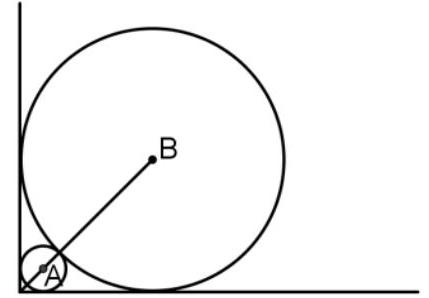
\includegraphics[max width=\textwidth, center]{2024_11_21_8e981e1ab2c7e641f462g-11}\\
okręgów do obwodu mniejszego jest równy \(3+2 \sqrt{2}\).

\begin{center}
\begin{tabular}{|c|c|c|c|c|c|c|c|c|c|c|c|c|c|c|c|c|c|c|c|c|c|c|c|c|c|c|c|c|c|c|c|}
\hline
 &  &  &  &  &  &  &  &  &  &  &  &  &  &  &  &  &  &  &  &  &  &  &  &  &  &  &  &  &  &  &  \\
\hline
 &  &  &  &  &  &  &  &  &  &  &  &  &  &  &  &  &  &  &  &  &  &  &  &  &  &  &  &  &  &  &  \\
\hline
 &  &  &  &  &  &  &  &  &  &  &  &  &  &  &  &  &  &  &  &  &  &  &  &  &  &  &  &  &  &  &  \\
\hline
 &  &  &  &  &  &  &  &  &  &  &  &  &  &  &  &  &  &  &  &  &  &  &  &  &  &  &  &  &  &  &  \\
\hline
 &  &  &  &  &  &  &  &  &  &  &  &  &  &  &  &  &  &  &  &  &  &  &  &  &  &  &  &  &  &  &  \\
\hline
 &  &  &  &  &  &  &  &  &  &  &  &  &  &  &  &  &  &  &  &  &  &  &  &  &  &  &  &  &  &  &  \\
\hline
 &  &  &  &  &  &  &  &  &  &  &  &  &  &  &  &  &  &  &  &  &  &  &  &  &  &  &  &  &  &  &  \\
\hline
 &  &  &  &  &  &  &  &  &  &  &  &  &  &  &  &  &  &  &  &  &  &  &  &  &  &  &  &  &  &  &  \\
\hline
 &  &  &  &  &  &  &  &  &  &  &  &  &  &  &  &  &  &  &  &  &  &  &  &  &  &  &  &  &  &  &  \\
\hline
 &  &  &  &  &  &  &  &  &  &  &  &  &  &  &  &  &  &  &  &  &  &  &  &  &  &  &  &  &  &  &  \\
\hline
 &  &  &  &  &  &  &  &  &  &  &  &  &  &  &  &  &  &  &  &  &  &  &  &  &  &  &  &  &  &  &  \\
\hline
 &  &  &  &  &  &  &  &  &  &  &  &  &  &  &  &  &  &  &  &  &  &  &  &  &  &  &  &  &  &  &  \\
\hline
 &  &  &  &  &  &  &  &  &  &  &  &  &  &  &  &  &  &  &  &  &  &  &  &  &  &  &  &  &  &  &  \\
\hline
 &  &  &  &  &  &  &  &  &  &  &  &  &  &  &  &  &  &  &  &  &  &  &  &  &  &  &  &  &  &  &  \\
\hline
 &  &  &  &  &  &  &  &  &  &  &  &  &  &  &  &  &  &  &  &  &  &  &  &  &  &  &  &  &  &  &  \\
\hline
 &  &  &  &  &  &  &  &  &  &  &  &  &  &  &  &  &  &  &  &  &  &  &  &  &  &  &  &  &  &  &  \\
\hline
 &  &  &  &  &  &  &  &  &  &  &  &  &  &  &  &  &  &  &  &  &  &  &  &  &  &  &  &  &  &  &  \\
\hline
 &  &  &  &  &  &  &  &  &  &  &  &  &  &  &  &  &  &  &  &  &  &  &  &  &  &  &  &  &  &  &  \\
\hline
 &  &  &  &  &  &  &  &  &  &  &  &  &  &  &  &  &  &  &  &  &  &  &  &  &  &  &  &  &  &  &  \\
\hline
\end{tabular}
\end{center}

Zadanie 29. (2 pkt)\\
Rozwiąż nierówność \(x^{2}-(3-x)(x+2) \geq 4\).\\

\includegraphics[max width=\textwidth, center]{2024_11_21_8e981e1ab2c7e641f462g-11(1)}

Zadanie 30. (2 pkt)\\
Oblicz wartość wyrażenia \(\frac{\sqrt{2} \cos \alpha-3 \sin \alpha}{4 \cos \alpha}\) wiedząc, że \(\operatorname{tg} \alpha=\sqrt{2}\) i \(\alpha \in\left(0^{\circ}, 90^{\circ}\right)\).\\

\includegraphics[max width=\textwidth, center]{2024_11_21_8e981e1ab2c7e641f462g-12}

Zadanie 31. (2 pkt)\\
Liczba naturalna \(n\) przy dzieleniu przez 5 daje resztę 3 , liczba \(m\) również przy dzieleniu przez 5 resztę 2 . Udowodnij, że reszta z dzielenia iloczynu liczb \(n \cdot m\) przez 5 daje resztę 1.\\
\(\qquad\)

Zadanie 32. (4 pkt)\\
W ostrosłupie prawidłowym czworokątnym \(A B C D S\) krawędź boczna ma długość 6, a kąt nachylenia ściany bocznej do płaszczyzny podstawy ostrosłupa ma miarę \(30^{\circ}\). Oblicz objętość tego ostrosłupa.\\

\includegraphics[max width=\textwidth, center]{2024_11_21_8e981e1ab2c7e641f462g-13}

Zadanie 33. (5 pkt)\\
Caąg \(\left(b_{n}\right)\) jest arytmetyczny i \(S_{60}-S_{39}=105\), gdzie \(S_{n}\) oznacza sumę \(n\) początkowych wyrazów tego ciągu. Oblicz \(x\), wiedząc, że liczby \(1,\left(b_{47}+b_{53}\right) x, 5 x+b_{50}\) tworzą rosnący ciąg geometryczny.\\

\includegraphics[max width=\textwidth, center]{2024_11_21_8e981e1ab2c7e641f462g-14}

Zadanie 34. (4 pkt)\\
Dany jest trójkąt \(A B C\), w którym \(A=(-2 ;-2)\) i \(B=(2 ; 1)\). Wierzchołek \(C\) leży na prostej o równaniu \(y=2 x-3\). Oblicz współzzędne wierzchołka \(C\), dla którego suma kwadratów długości boków trójkąta jest najmniejsza.

\begin{center}
\begin{tabular}{|c|c|c|c|c|c|c|c|c|c|c|c|c|c|c|c|c|c|c|c|c|c|c|}
\hline
 &  &  &  &  &  &  &  &  &  &  &  &  &  &  &  &  &  &  &  &  &  &  \\
\hline
 &  &  &  &  &  &  &  &  &  &  &  &  &  &  &  &  &  &  &  &  &  &  \\
\hline
 &  &  &  &  &  &  &  &  &  &  &  &  &  &  &  &  &  &  &  &  &  &  \\
\hline
 &  &  &  &  &  &  &  &  &  &  &  &  &  &  &  &  &  &  &  &  &  &  \\
\hline
 &  &  &  &  &  &  &  &  &  &  &  &  &  &  &  &  &  &  &  &  &  &  \\
\hline
 &  &  &  &  &  &  &  &  &  &  &  &  &  &  &  &  &  &  &  &  &  &  \\
\hline
 &  &  &  &  &  &  &  &  &  &  &  &  &  &  &  &  &  &  &  &  &  &  \\
\hline
 &  &  &  &  &  &  &  &  &  &  &  &  &  &  &  &  &  &  &  &  &  &  \\
\hline
 &  &  &  &  &  &  &  &  &  &  &  &  &  &  &  &  &  &  &  &  &  &  \\
\hline
 &  &  &  &  &  &  &  &  &  &  &  &  &  &  &  &  &  &  &  &  &  &  \\
\hline
 &  &  &  &  &  &  &  &  &  &  &  &  &  &  &  &  &  &  &  &  &  &  \\
\hline
 &  &  &  &  &  &  &  &  &  &  &  &  &  &  &  &  &  &  &  &  &  &  \\
\hline
 &  &  &  &  &  &  &  &  &  &  &  &  &  &  &  &  &  &  &  &  &  &  \\
\hline
 &  &  &  &  &  &  &  &  &  &  &  &  &  &  &  &  &  &  &  &  &  &  \\
\hline
 &  &  &  &  &  &  &  &  &  &  &  &  &  &  &  &  &  &  &  &  &  &  \\
\hline
 &  &  &  &  &  &  &  &  &  &  &  &  &  &  &  &  &  &  &  &  &  &  \\
\hline
 &  &  &  &  &  &  &  &  &  &  &  &  &  &  &  &  &  &  &  &  &  &  \\
\hline
 &  &  &  &  &  &  &  &  &  &  &  &  &  &  &  &  &  &  &  &  &  &  \\
\hline
 &  &  &  &  &  &  &  &  &  &  &  &  &  &  &  &  &  &  &  &  &  &  \\
\hline
 &  &  &  &  &  &  &  &  &  &  &  &  &  &  &  &  &  &  &  &  &  &  \\
\hline
 &  &  &  &  &  &  &  &  &  &  &  &  &  &  &  &  &  &  &  &  &  &  \\
\hline
 &  &  &  &  &  &  &  &  &  &  &  &  &  &  &  &  &  &  &  &  &  &  \\
\hline
 &  &  &  &  &  &  &  &  &  &  &  &  &  &  &  &  &  &  &  &  &  &  \\
\hline
 &  &  &  &  &  &  &  &  &  &  &  &  &  &  &  &  &  &  &  &  &  &  \\
\hline
 &  &  &  &  &  &  &  &  &  &  &  &  &  &  &  &  &  &  &  &  &  &  \\
\hline
 &  &  &  &  &  &  &  &  &  &  &  &  &  &  &  &  &  &  &  &  &  &  \\
\hline
 &  &  &  &  &  &  &  &  &  &  &  &  &  &  &  &  &  &  &  &  &  &  \\
\hline
 &  &  &  &  &  &  &  &  &  &  &  &  &  &  &  &  &  &  &  &  &  &  \\
\hline
 &  &  &  &  &  &  &  &  &  &  &  &  &  &  &  &  &  &  &  &  &  &  \\
\hline
 &  &  &  &  &  &  &  &  &  &  &  &  &  &  &  &  &  &  &  &  &  &  \\
\hline
 &  &  &  &  &  &  &  &  &  &  &  &  &  &  &  &  &  &  &  &  &  &  \\
\hline
 &  &  &  &  &  &  &  &  &  &  &  &  &  &  &  &  &  &  &  &  &  &  \\
\hline
 &  &  &  &  &  &  &  &  &  &  &  &  &  &  &  &  &  &  &  &  &  &  \\
\hline
 &  &  &  &  &  &  &  &  &  &  &  &  &  &  &  &  &  &  &  &  &  &  \\
\hline
 &  &  &  &  &  &  &  &  &  &  &  &  &  &  &  &  &  &  &  &  &  &  \\
\hline
 &  &  &  &  &  &  &  &  &  &  &  &  &  &  &  &  &  &  &  &  &  &  \\
\hline
 &  &  &  &  &  &  &  &  &  &  &  &  &  &  &  &  &  &  &  &  &  &  \\
\hline
 &  &  &  &  &  &  &  &  &  &  &  &  &  &  &  &  &  &  &  &  &  &  \\
\hline
 &  &  &  &  &  &  &  &  &  &  &  &  &  &  &  &  &  &  &  &  &  &  \\
\hline
 &  &  &  &  &  &  &  &  &  &  &  &  &  &  &  &  &  &  &  &  &  &  \\
\hline
 &  &  &  &  &  &  &  &  &  &  &  &  &  &  &  &  &  &  &  &  &  &  \\
\hline
 &  &  &  &  &  &  &  &  &  &  &  &  &  &  &  &  &  &  &  &  &  &  \\
\hline
\end{tabular}
\end{center}

\begin{center}

\includegraphics[max width=\textwidth]{2024_11_21_8e981e1ab2c7e641f462g-16}
\end{center}

Odpowiedź:

\section*{PESEL}
WYPEŁNIA ZDAJĄCY

\begin{center}
\begin{tabular}{|c|c|c|c|c|}
\hline
\multirow{2}{*}{\begin{tabular}{l}
Nr \\
zad. \\
\end{tabular}} & \multicolumn{4}{|c|}{Odpowiedzi} \\
\hline
 & A & B & C & D \\
\hline
1 & ㅁ & ㅁ & - & ■ \\
\hline
2 & ㅁ & \(\square\) & - & \(\square\) \\
\hline
3 & ㅁ & ㅁ & ■ & \(\square\) \\
\hline
4 & ㅁ & \(\square\) & - & \(\square\) \\
\hline
5 & ㅁ & \(\square\) & - & \(\square\) \\
\hline
6 & ㅁ & ㅁ & - & \(\square\) \\
\hline
7 & ㅁ & ㅁ & ■ & \(\square\) \\
\hline
8 & ㅁ & ㅁ & ■ & \(\square\) \\
\hline
9 & ㅁ & ㅁ & ■ & \(\square\) \\
\hline
10 & ■ & ■ & - & \(\square\) \\
\hline
11 & - & ㅁ & - & \(\square\) \\
\hline
12 & ㅁ & ㅁ & ㅁ & \(\square\) \\
\hline
13 & ㅁ & ㅁ & ■ & \(\square\) \\
\hline
14 & ㅁ & ㅁ & ■ & ㅁ \\
\hline
15 & ㅁ & \(\square\) & ■ & \(\square\) \\
\hline
16 & ㅁ & \(\square\) & - & \(\square\) \\
\hline
17 & ㅁ & ■ & ■ & \(\square\) \\
\hline
18 & ㅁ & ㅁ & ■ & \(\square\) \\
\hline
19 & ㅁ & ㅁ & \(\square\) & \(\square\) \\
\hline
20 & ■ & \(\square\) & ■ & \(\square\) \\
\hline
21 & ㅁ & ㅁ & \(\square\) & \(\square\) \\
\hline
22 & ㅁ & ■ & - & \(\square\) \\
\hline
23 & ㅁ & ㅁ & - & \(\square\) \\
\hline
24 & ㅁ & ㅁ & ㅁ & \(\square\) \\
\hline
25 & ㅁ & ㅁ & - & \(\square\) \\
\hline
\end{tabular}
\end{center}

WYPEŁNIA EGZAMINATOR

\begin{center}
\begin{tabular}{|c|c|c|c|c|c|c|}
\hline
\multirow{2}{*}{\begin{tabular}{c}
Nr \\
zad. \\
\end{tabular}} & \multicolumn{6}{|c|}{Punkty} \\
\hline
 & \(\mathbf{1}\) & \(\mathbf{2}\) & \(\mathbf{3}\) & \(\mathbf{4}\) & \(\mathbf{5}\) &  \\
\hline
\(\mathbf{2 6}\) & \(\square\) & \(\square\) & \(\square\) &  &  &  \\
\hline
\(\mathbf{2 7}\) & \(\square\) & \(\square\) & \(\square\) &  &  &  \\
\hline
\(\mathbf{2 8}\) & \(\square\) & \(\square\) & \(\square\) &  &  &  \\
\hline
\(\mathbf{2 9}\) & \(\square\) & \(\square\) & \(\square\) &  &  &  \\
\hline
\(\mathbf{3 0}\) & \(\square\) & \(\square\) & \(\square\) &  &  &  \\
\hline
\(\mathbf{3 1}\) & \(\square\) & \(\square\) & \(\square\) &  &  &  \\
\hline
\(\mathbf{3 2}\) & \(\square\) & \(\square\) & \(\square\) & \(\square\) & \(\square\) &  \\
\hline
\(\mathbf{3 3}\) & \(\square\) & \(\square\) & \(\square\) & \(\square\) & \(\square\) & \(\square\) \\
\hline
\(\mathbf{3 4}\) & \(\square\) & \(\square\) & \(\square\) & \(\square\) & \(\square\) &  \\
\hline
\end{tabular}
\end{center}

SUMA\\
PUNKTÓW\\

\includegraphics[max width=\textwidth, center]{2024_11_21_8e981e1ab2c7e641f462g-17}


\end{document}